\section{Application}
\label{sec:application}

This Section will further outline the use case of Partial
Classification and the PCF, displaying results of a test on
an artificial dataset and comparing the PCF to other,
non-partial classifiers. Furthermore a test of the
PCF's behavior with different amounts of Trees will be
shown.

Both tests are performed on a randomly generated,
normalized, two dimensional and binary labeled dataset. The
dataset contains five thousand observations and was
designed to be unpredictable, when predicted as a whole.
The plane from which the observations are generated
contains five partitions in which the observations all have
the same label. Observations from those five partitions
make up twenty percent of all observations and are the only
ones which should be predicted, because all points not
inside those partitions are labeled randomly. The optimal
decision surface would be equal to the area of the five
partitions.

All observations are generated by a pseudo-random number
generator\cite[chapter 9.6]{python}, therefore: every point
on the plane has the same probability to be chosen as an
observation for the dataset.

The dataset is designed this way in order to be able to
show the application of the PCF in the domain of Partial
Classification. Only twenty percent of the whole dataset is
predictable which makes it impossible for other,
non-partial classifiers to be able to find an adequate
decision surface (see Figure~\ref{fig:other_classif}). The
following tests all take $\tau_l = 1$ as quality threshold
which is impossible to achieve predicting on the whole
dataset.

It is common practice in machine learning to split a
dataset into a training and a test set in order to find
the best model.\cite[chapter 18]{ki}
This approach is also used for the PCF. The training set is
used as the parameters $X$ and $y$ of FIT (Algorithm~%
\ref{alg:pcf_fit}) while PREDICT (Algorithm~%
\ref{alg:pcf_pred}) is used on every observation of the
test set.

Two metrics are used to describe the behavior of the PCF,
(\romannumeral 1) $predicted$ and (\romannumeral 2)
$accuracy$. Both metrics are derived from comparing the
label of an observation returned by PREDICT with its actual
label from the dataset.

$Predicted$ is the percentage of predicted observations,
while $accuracy$ is the percentage of correctly classified
observations from the test set. $Accuracy$ is used as the
quality measurement, which means in the context of this
tests, every classifier not able to achieve $accuracy = 1$
when predicting the test set does not solve the
classification problem.

For both tests $\gamma$, $\tau_l$ and $\tau_h$ are the
same. $\gamma$ and $\tau_l$ are equal to the values used in
Figure~\ref{fig:fit_example} while $\tau_h$ equals 32. The
dataset was split into a training and a test set such
that ten percent of the observations were used as the test
set.\footnote{For splitting scikit-learn's
  model\_selection.train\_test\_split was used during the
  tests.\cite{sklearn_api}} The observations for the test
set were chosen randomly.

The first test will show the decision surfaces of PCF
instances with different $N$ and $\tau_{|X|}$. For the test
three different values, two, five and ten were used for
both $N$ and $\tau_{|X|}$ to show how those two parameters
change the decision surface of the PCF instances. The test
shows that for $\tau_{|X|} = 2$ the PCF instances
over-fitted the data, $predicted$ exceeding twenty percent
--- the amount of accurate observations --- while
$accuracy$ fails to equal $\tau_l$. This results in the
chaotic decision surfaces shown in Figures~\ref{fig:x2_n2}
- \ref{fig:x2_n10}. On the other hand for $\tau{|X|} = 10$
the decision surface is very small which means the PCF
instances' $predicted$ is far less than twenty percent
(Figures~\ref{fig:x10_n2} - \ref{fig:x10_n10}).

How non-partial classifiers perform on the dataset can be
seen in Figure~\ref{fig:other_classif}. Three common
classifiers are tested, all from the scikit-learn library
(version 0.20.1).\cite{sklearn_api}
Their parameters are the standard parameters given by
scikit-learn. Tested were the Support Vector Machine,
Random Forest and K Nearest Neighbors, where K in this case
equals five.\cite{sklearn_api}
Figure~\ref{fig:other_classif} also shows the $accuracy$ of
these classifiers. None are close to $\tau_l = 1$.

The second test shows the influence the amount of Trees $N$
has on $predicted$ and $accuracy$. In this test
$\tau_{|X|}$ equals four.

Figure~\ref{fig:n} shows: for this dataset with the
chosen thresholds the PCF instances with $N < 30$ variate,
both their $predicted$ and $accuracy$ values. Is $30 \leq N
\leq 100$ $accuracy$ is constant and equals $\tau_l$.
$Predicted$ on the other hand still rises in this
interval. Is $N \geq 100$ $predicted$ is higher than
$predicted$ with $N = 100$ and constant, but $accuracy$
fails to meet $\tau_l$, which means the PCF instances are
over-fitting.

Furthermore the second test relates $predicted$ and
$accuracy$ of the observations from the test set to the
values for the training set, showing that more training
observations are predictable than test observations
(see Figure~\ref{fig:n}).

\def\setmeshr#1{
  \def\meshr{#1}
}
\def\meshr{1pt}

\pgfooclass{meshgrid visualizer}{
  % Stores the name of the visualizer. This is needed for
  % filtering and configuration
  \attribute name;

  % The constructor. Just setup the attribute.
  \method meshgrid visualizer(#1) { \pgfooset{name}{#1} }

  % Connect to visualize signal.
  \method default connects() {
    \pgfoothis.get handle(\me)
    \pgfkeysvalueof{/pgf/data visualization/obj}.connect(
      \me,visualize,visualize datapoint signal)
  }

  % This method is invoked for each data point. It checks
  % whether the data point belongs to the correct
  % visualizer and, if so, calls the macro \dovisualization
  % to do the actual visualization.
  \method visualize() {
    \pgfdvfilterpassedtrue
    \pgfdvnamedvisualizerfilter
    \ifpgfdvfilterpassed
      \dovisualization
    \fi
  }
}

\def\dovisualization{
  \pgfkeysvalueof{%
    /data point/\pgfoovalueof{name}/execute at begin%
  }

  \pgfpointdvdatapoint
  \pgfgetlastxy{\macrox}{\macroy}

  \pgfmathsetmacro\xlow {\macrox - \meshr}
  \pgfmathsetmacro\ylow {\macroy - \meshr}
  \pgfmathsetmacro\xhigh{\macrox + \meshr}
  \pgfmathsetmacro\yhigh{\macroy + \meshr}

  \pgfpathrectanglecorners{\pgfpoint{\xlow}{\ylow}}
                          {\pgfpoint{\xhigh}{\yhigh}}

  \pgfkeysvalueof{%
    /data point/\pgfoovalueof{name}/execute at end%
  }
}
\tikzdatavisualizationset{
  visualize as meshgrid/.style={
    new object={
      when=after survey,
      store=/tikz/data visualization/visualizers/#1,
      class=meshgrid visualizer,
      arg1=#1
    },
    new visualizer={#1}{%
      color=visualizer color,
      every path/.style={fill,draw,opacity=0.5},
    }{},
    /data point/set=#1
  },
  visualize as meshgrid/.default=meshgrid
}

\setmeshr{0.5pt}

\def\visualizeds#1{
  \begin{tikzpicture}
    \datavisualization [
      scientific axes=clean,
      visualize as meshgrid/.list={mesh0, mesh1},
      visualize as scatter/.list={data0, data1},
      x axis={label={$x_0$}},
      y axis={label={$x_1$}},
      mesh0={style={color=red!50}},
      mesh1={style={color=blue!50}},
      data0={style={mark=o, mark size=0.1pt,
        visualizer color=red}},
      data1={style={mark=o, mark size=0.1pt,
        visualizer color=blue}},
    ]
    data[headline={x, y}, read from file=#1.mesh_0.csv,
      set=mesh0]
    data[headline={x, y}, read from file=#1.mesh_1.csv,
      set=mesh1]
    data[headline={x, y}, read from file=#1.data_0.csv,
      set=data0]
    data[headline={x, y}, read from file=#1.data_1.csv,
      set=data1]
    ;
  \end{tikzpicture}
}

\def\dslegend{
  \begin{flushright}
    \begin{tikzpicture}
      \begin{scope}[label distance=2pt]
        \node[color=red, circle, draw,fill,
          label=right:label 0, inner sep=1.5pt] at (0,0)
            (l_zero) {};
        \node[color=blue, circle,draw,fill,
          label=right:label 1, below=0.2 of l_zero,
          inner sep=1.5pt] (l_one) {};
      \end{scope}

      \node[color=red!50,opacity=0.5,
        label=right:predicted 0, below=0.2 of l_one, fill,
        draw] (m_zero) {};
      \node[color=blue!50,opacity=0.5,below=0.2 of m_zero,
        label=right:predicted 1, fill, draw] (m_one) {};
    \end{tikzpicture}
  \end{flushright}
}

% decision surface figure {{{
\begin{figure*}
  \begin{comment}
  \begin{subfigure}[b]{0.3\textwidth}
    \centering
    \scalebox{0.7}{%
      \visualizeds{application/data/decision_surface/e2_ls2}}
    \caption{}
    \vspace{-0.5cm}
    \begin{align*}
      \tau_{|X|} = 2&, N = 2, \\
      predicted &= 0.37
, \\
      accuracy &= 0.670

    \end{align*}
    \label{fig:x2_n2}
  \end{subfigure}
  \begin{subfigure}[b]{0.3\textwidth}
    \centering
    \scalebox{0.7}{%
      \visualizeds{application/data/decision_surface/e5_ls2}}
    \caption{}
    \vspace{-0.5cm}
    \begin{align*}
      \tau_{|X|} = 2&, N = 5, \\
      predicted &= 0.308
, \\
      accuracy &= 0.721

    \end{align*}
    \label{fig:x2_n5}
  \end{subfigure}
  \begin{subfigure}[b]{0.3\textwidth}
    \centering
    \scalebox{0.7}{%
      \visualizeds{application/data/decision_surface/e10_ls2}}
    \caption{}
    \vspace{-0.5cm}
    \begin{align*}
      \tau_{|X|} = 2&, N = 10, \\
      predicted &= 0.298
, \\
      accuracy &= 0.792

    \end{align*}
    \label{fig:x2_n10}
  \end{subfigure}

  \begin{subfigure}[b]{0.3\textwidth}
    \centering
    \scalebox{0.7}{%
      \visualizeds{application/data/decision_surface/e2_ls5}}
    \caption{}
    \vspace{-0.5cm}
    \begin{align*}
      \tau_{|X|} = 5&, N = 2, \\
      predicted &= 0.144
, \\
      accuracy &= 0.903

    \end{align*}
  \end{subfigure}
  \begin{subfigure}[b]{0.3\textwidth}
    \centering
    \scalebox{0.7}{%
      \visualizeds{application/data/decision_surface/e5_ls5}}
    \caption{}
    \vspace{-0.5cm}
    \begin{align*}
      \tau_{|X|} = 5&, N = 5, \\
      predicted &= 0.106
, \\
      accuracy &= 0.962

    \end{align*}
  \end{subfigure}
  \begin{subfigure}[b]{0.3\textwidth}
    \centering
    \scalebox{0.7}{%
      \visualizeds{application/data/decision_surface/e10_ls5}}
    \caption{}
    \vspace{-0.5cm}
    \begin{align*}
      \tau_{|X|} = 5&, N = 10, \\
      predicted &= 0.138, \\
      accuracy &= 1

    \end{align*}
  \end{subfigure}

  \begin{subfigure}[b]{0.3\textwidth}
    \centering
    \scalebox{0.7}{%
      \visualizeds{application/data/decision_surface/e2_ls10}}
    \caption{}
    \vspace{-0.5cm}
    \begin{align*}
      \tau_{|X|} = 10&, N = 2, \\
      predicted &= 0.076
, \\
      accuracy &= 1

    \end{align*}
    \label{fig:x10_n2}
  \end{subfigure}
  \begin{subfigure}[b]{0.3\textwidth}
    \centering
    \scalebox{0.7}{%
      \visualizeds{application/data/decision_surface/e5_ls10}}
    \caption{}
    \vspace{-0.5cm}
    \begin{align*}
      \tau_{|X|} = 10&, N = 5, \\
      predicted &= 0.074
, \\
      accuracy &= 1

    \end{align*}
    \label{fig:x10_n5}
  \end{subfigure}
  \begin{subfigure}[b]{0.3\textwidth}
    \centering
    \scalebox{0.7}{%
      \visualizeds{application/data/decision_surface/e10_ls10}}
    \caption{}
    \vspace{-0.5cm}
    \begin{align*}
      \tau_{|X|} = 10&, N = 10, \\
      predicted &= 0.068
, \\
      accuracy &= 1

    \end{align*}
    \label{fig:x10_n10}
  \end{subfigure}
  \end{comment}

  \dslegend

  \caption{The decision surfaces of differently configured
    PCF instances. The threshold $\tau_{|X|}$ and the
    amount of Trees $N$ are different for each Figure,
    \ref{fig:x2_n2} - \ref{fig:x10_n10}.}
  \label{fig:decision_surface}
\end{figure*}
% }}}

\begin{figure*}
  \begin{comment}
  \begin{subfigure}[b]{0.3\textwidth}
    \centering
    \scalebox{0.7}{%
      \visualizeds{application/data/other_classif/svm}}
    \caption{Support Vector Machine.}
    \vspace{-0.5cm}
    \begin{align*}
      Accuracy = 0.554
    \end{align*}
  \end{subfigure}
  \begin{subfigure}[b]{0.3\textwidth}
    \centering
    \scalebox{0.7}{%
      \visualizeds{application/data/other_classif/rf}}
    \caption{Random Forest.}
    \vspace{-0.5cm}
    \begin{align*}
      Accuracy = 0.596
    \end{align*}
  \end{subfigure}
  \begin{subfigure}[b]{0.3\textwidth}
    \centering
    \scalebox{0.7}{%
      \visualizeds{application/data/other_classif/nn}}
    \caption{K Nearest Neighbor.}
    \vspace{-0.5cm}
    \begin{align*}
      Accuracy = 0.56
    \end{align*}
  \end{subfigure}
  \end{comment}

  \dslegend

  \caption{The decision surfaces of non-partial
    classifiers.}
  \label{fig:other_classif}
\end{figure*}


\begin{figure*}
  \begin{subfigure}[b]{0.5\textwidth}
    \begin{tikzpicture}
      \datavisualization [
        scientific axes=clean,
        x axis={label={$N$}},
        y axis={label={Predicted}},
        visualize as line/.list={fit, pred},
        fit={style={color=red}},
        pred={style={color=blue}},
      ]
      data[headline={x, y}, read from file=tests/data/fit_known_4.csv,
        set=fit]
      data[headline={x, y}, read from file=tests/data/pred_known_4.csv,
        set=pred]
      ;
    \end{tikzpicture}
  \end{subfigure}
  \begin{subfigure}[b]{0.5\textwidth}
    \begin{tikzpicture}
      \datavisualization [
        scientific axes=clean,
        x axis={label={$N$}},
        y axis={label={Accuracy}},
        visualize as line/.list={fit, pred},
        fit={style={color=red}},
        pred={style={color=blue}},
      ]
      data[headline={x, y}, read from file=tests/data/fit_acc_4.csv,
        set=fit]
      data[headline={x, y}, read from file=tests/data/pred_acc_4.csv,
        set=pred]
      ;
    \end{tikzpicture}
  \end{subfigure}
  \begin{flushright}
    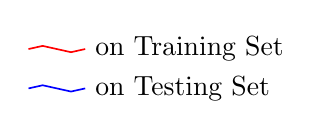
\begin{tikzpicture}
      \draw[red,semithick] (0,.5) -- (.18,.54) --
        (.54,.46) -- (.72,.5) node[right,black]
        {on Training Set};
      \draw[blue,semithick] (0,0) -- (.18,.04) --
        (.54,-.04) -- (.72,0) node[right,black]
        {on Testing Set};
    \end{tikzpicture}
  \end{flushright}
\end{figure*}


